\section{Convolutional neural networks (CNN) für Graphen}

\subsection{Einleitung}

\begin{itemize}
  \item \underline{Anwendungsfälle:}
  \begin{enumerate}
    \item Aus einer Menge von Graphen soll eine Funktion für Klassifizierungs- oder Regressionsprobleme gelernt werden, die auf nicht bekannte Graphen angewendet werden kann
    \item lerne Graph-Repräsentationen, um auf Graph-Eigenschaften (fehlende Kanten, Knoteneigenschaften) unbekannter Graphen zu schließen
  \end{enumerate}
\item \underline{Graphrepräsentation:}
  \begin{itemize}
    \item Graphen können gerichtet oder ungerichtet sein
    \item Graphen können zyklisch sein
    \item Graphen können mehrere unterschiedliche Kantentypen besitzen (mehrere Perceptive-Field-Layer)
    \item Graphen können mehrere diskrete oder kontinuierliche Werte an ihren Knoten haben
  \end{itemize}
\item Methode berechnet lokal verbundene Nachbarschaften der Graphen und benutzt sie als die \emph{Receptive Fields} des CNN
\item die Methode kann für Graphen mit gewichteten Kanten erweitert werden
\end{itemize}

\begin{figure}[h]
  \centering
  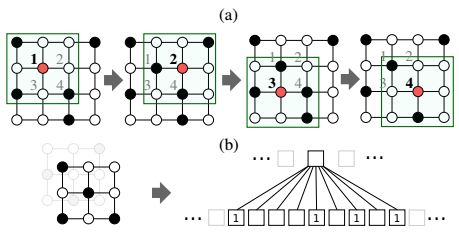
\includegraphics[width=.5\textwidth]{images/cnn_graph.png}
\end{figure}

\begin{itemize}
  \item \underline{Idee:} repräsentiere Bilder als Graph
    \begin{itemize}
      \item ein Bild kann als Graph repräsentiert werden, indem die Knoten jeweils einen Pixel repräsentieren und es eine Kante zwischen zwei Knoten gibt, wenn deren Pixel benachbart sind
      \item die lokale Nachbarschaft eines Pixels wird repräsentiert als ein Quadrat um den Punkt (hier $3 \times 3$)
      \item Aus der Nachbarschaft kann ein Merkmal ermittelt werden
    \end{itemize}
  \item üblicherweise gibt es keine räumliche Anordnung einer Graph-Repräsentation
  \item \underline{Probleme:}
    \begin{enumerate}
      \item Welche Nachbarschaften um welche Knoten und in welcher Reihenfolge bilden die Receptive Fiels?
      \item Wie können die einzelnen Nachbarschafts-Graphen in einem Vektor repräsentiert werden (Normalisierung)?
    \end{enumerate}
  \item \underline{Verfahren:}
    \begin{enumerate}
      \item bestimme eine Knoten-Auswahl inklusive Reihenfolge
      \item bestimme den Nachbarschafts-Graphen um diesen Knoten mit genau $k$ Knoten
      \item normalisiere die Nachbarschafts-Graphen
      \item füttere sie in ein CNN
    \end{enumerate}
\end{itemize}

\subsection{Grundlagen}

\begin{itemize}
  \item Graph $G = (V, E)$ mit $V = \lbrace v_1, \ldots, v_n \rbrace$ und $E \subseteq V \times V$, wobei $n$ Anzahl der Knoten und $m$ Anzahl der Kanten
  \item Adjazenzmatrix $A$ mit Größe $n \times n$, wobei $A_{i,j} = 1$, falls eine Kante von $v_i$ nach $v_j$ existiert (sonst $0$) $\Rightarrow$ $v_i$ und $v_j$ sind adjazent
  \item ein Weg ist eine Sequenz von Knoten, bei der benachbarte Knoten adjazent sind
  \item $d(u,v)$ beschreibt die minimale Distanz zwischen von $u$ nach $v$
  \item $N_1(v)$ beschreibt die 1-Nachbarschaft um einen Knoten, d.h.\ alle Knoten die adjazent sind zu $v$
\end{itemize}

\subsubsection{Beschriftung und Partitionierung}

\begin{itemize}
  \item eine Graph-Beschriftung $l: V \rightarrow S$ bildet einen Knoten auf eine sortierbare Einheit ab
  \item induziert ein \emph{Ranking} $r: V \rightarrow \lbrace 1, \ldots, |V| \rbrace$ mit $r(u) < r(v)$ genau dann, wenn $l(u) > l(v)$
  \item falls $l$ injektiv, dann gibt es eine totale Ordnung der Knoten in $G$ und eine eindeutige Adjazenzmatrix $A^l$, bei der die Knoten die Position $r(v)$ haben
  \item eine Graph-Beschriftung induziert eine Partionierung $\lbrace V_1, \ldots V_k \rbrace$ mit $u, v \in V_i$ falls $l(u) = l(v)$
  \item \underline{Metriken:}
    \begin{itemize}
      \item Anteil an kürzesten Wegen von $v$ zu $v$ (\emph{Betweeness centrality})
      \item Grad der Knoten (Anzahl adjazenter Knoten)
      \item \ldots
    \end{itemize}
\end{itemize}

\subsection{Lernen von Graphen}

\subsubsection{Knotenauswahl}

\begin{itemize}
  \item Auswahl an Knoten, für die ein Receptive Field erstellt werden soll
  \item \underline{Gegeben:} Graph-Beschreibung $l$, Abstand $s$, Anzahl $w$ an Reciptive Fields
\end{itemize}

\begin{enumerate}
  \item sortiere die Knoten auf Basis von $l$
  \item iteriere über die sortierte Knotenmenge mit Abständen $s$, bis $w$ Knoten ausgewählt wurden
\end{enumerate}

\subsubsection{Nachbarschaftssuche}

\begin{itemize}
  \item \underline{Gegeben:} Knoten $v$, Größe $k$ des Receptive Fields
\end{itemize}

\begin{enumerate}
  \item setze initiale Knotenmenge $N$ auf $v$
  \item wiederhole bis $|N| > k$:
    \begin{enumerate}
      \item berechne für alle Knoten $i$ in $N$ die Nachbarschaften $N_1(i)$ und füge sie zu $N$ hinzu
    \end{enumerate}
\end{enumerate}

\begin{itemize}
  \item \underline{Bemerkung:} im Allgemein gilt $|N| \neq k$
\end{itemize}

\subsubsection{Normalisierung}

\begin{itemize}
  \item \underline{Gegeben:} Menge von Graphen $\mathcal{G}$ mit $k$ Knoten, Distanzmetriken für Matrizen $d_A$ und Graphen $d_G$
  \item \underline{Optimierungsproblem:} $\min_l \sum_{G \in \mathcal{G}} \sum_{G' \in \mathcal{G}} {( d_A(A^l(G), A^l(G') - d_g(G, G')) )}$

\end{itemize}

\subsection{Auswertung}

\begin{itemize}
  \item CNNs mit Bildern können identisch über CNNs mit Graphen dargestellt werden
  \item Methode funktioniert teilweise deutlich besser als State-of-the-Art Graph-Kerne (z.B.\ bei Klasifizierungsproblemen)
\end{itemize}

\subsection{Zukünftige Arbeiten}

\begin{itemize}
  \item gewichtete Kanten (oder allgemein mit Kanteneigenschaften)
  \item Graphen auf andere Netze übertragen, z.B.\ RNNs
  \item kombiniere unterschiedliche Receptive Field Größen
\end{itemize}
